\section*{Module description}
\begin{tabularx}{\textwidth}{|>{\columncolor{lichtGrijs}} p{.26\textwidth}|X|}
	\hline
	\textbf{Module name:} & \modulenaam\\
	\hline
	\textbf{Module code: }& \modulecode\\
	\hline
	\textbf{Number of ECTS \newline and number of individual study hours:} & This module gives \stdPunten ECTS, which corresponds to 56 hours.
	\begin{itemize}
		\item 5 $\times$ 120 minutes frontal lecture
		\item 3 $\times$ 120 minutes practicum
		\item the rest is individual study
	\end{itemize} \\
	\hline
	\textbf{Examination:} & Practical assignments \\
	\hline
	\textbf{Course structure:} & Lectures and practicums \\
	\hline
	\textbf{Required knowledge:} & All programming course, linear algebra. \\
	\hline
	\textbf{Learning tools:}  &
		\begin{itemize}
			\item Book: Game Physics, author: David Eberly
			\item Book: Friendly F\# (Fun with game physics), authors: Giuseppe Maggiore, Marijn Tamis, Giulia Costantini
			\item Text editors: Emacs, Notepad++, Visual Studio, Xamarin Studio, etc.
		\end{itemize} \\
	\hline
	\textbf{Connects to \newline competencies :} &
	\begin{center}
		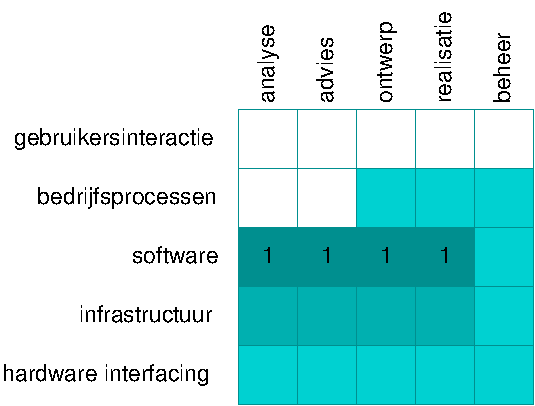
\includegraphics[width=7cm]{img/comptabel.pdf}
	\end{center}\\
	\hline
\end{tabularx}
\newpage

\begin{tabularx}{\textwidth}{|>{\columncolor{lichtGrijs}} p{.26\textwidth}|X|}
	\hline
	\textbf{Overall learning goal:}&
		The student is able to describe, define, and then implement numerical approximation techniques to physics simulations. \\
	\hline
	\textbf{Detailed learning goals:}&
	\begin{itemize}
		\item The student is able to distinguish the aspect of kinematics: linear and rotational motion, and associated forces (learning goal \textit{analysis});
		\item The student is able to give advice over the design and realisation of a kinematics simulation (learning goal \textit{advice});
		\item The student is able to design the structure and architecture of a kinematics simulation (learning goal \textit{design});
		\item The student is able to realise a working kinematics simulation (learning goal \textit{realisation});
		\item The student is able to communicate in correct Dutch or English, using the correct jargon, about physics simulations and kinematics, etc. (learning goal \textit{communication}).
	\end{itemize}
	\ \\
	\hline
	\textbf{Module responsible:} & \author\\
	\hline
	\textbf{Date:} & \today \\
	\hline
\end{tabularx}
\newpage
